% -----------------------------*- LaTeX -*------------------------------
\documentclass[12pt]{report}
\usepackage{sparsity_structures_and_algorithms_10, epsfig}
\usepackage{amsmath}
% Use something like:
% % Use something like:
% % Use something like:
% \input{../../macros}

% groupings of objects.
\newcommand{\set}[1]{\ensuremath{\left\{ #1 \right\}}}
\newcommand{\seq}[1]{\ensuremath{\left(#1\right)}}
\newcommand{\ang}[1]{\ensuremath{\langle#1\rangle}}
\newcommand{\tuple}[1]{\ensuremath{\left(#1\right)}}
\newcommand{\size}[1]{\ensuremath{\left| #1\right|}}

% numerical shortcuts.
\newcommand{\abs}[1]{\ensuremath{\left| #1\right|}}
\newcommand{\floor}[1]{\ensuremath{\left\lfloor #1 \right\rfloor}}
\newcommand{\ceil}[1]{\ensuremath{\left\lceil #1 \right\rceil}}

% linear algebra shortcuts.
\newcommand{\change}{\ensuremath{\Delta}}
\newcommand{\norm}[1]{\ensuremath{\left\| #1\right\|}}
\newcommand{\dprod}[1]{\ensuremath{\langle#1\rangle}}
\newcommand{\linspan}[1]{\ensuremath{\langle#1\rangle}}
\newcommand{\conj}[1]{\ensuremath{\overline{#1}}}
\newcommand{\der}{\ensuremath{\frac{d}{dx}}}
\newcommand{\lap}{\ensuremath{\Delta}}
\newcommand{\kron}{\ensuremath{\otimes}}
\newcommand{\nperp}{\ensuremath{\nvdash}}

\newcommand{\mat}[1]{\left[ \begin{smallmatrix}#1 \end{smallmatrix} \right]}

% derivatives and limits
\newcommand{\partder}[2]{\ensuremath{\frac{\partial #1}{\partial #2}}}
\newcommand{\partdern}[3]{\ensuremath{\frac{\partial^{#3} #1}{\partial #2^{#3}}}}
\newcommand{\gradient}{\ensuremath{\nabla}}
\newcommand{\subdifferential}{\ensuremath{\partial}}

% Arrows
\newcommand{\diverge}{\ensuremath{\nearrow}}
\newcommand{\notto}{\ensuremath{\nrightarrow}}
\newcommand{\up}{\ensuremath{\uparrow}}
\newcommand{\down}{\ensuremath{\downarrow}}
% gets and gives are defined!

% ordering operators
\newcommand{\oleq}{\preceq}
\newcommand{\ogeq}{\succeq}

% programming and logic operators
\newcommand{\dfn}{:=}
\newcommand{\assign}{:=}
\newcommand{\co}{\ co\ }
\newcommand{\en}{\ en\ }


% logic operators
\newcommand{\xor}{\ensuremath{\oplus}}
\newcommand{\Land}{\ensuremath{\bigwedge}}
\newcommand{\Lor}{\ensuremath{\bigvee}}
\newcommand{\finish}{\ensuremath{\Box}}
\newcommand{\contra}{\ensuremath{\Rightarrow \Leftarrow}}
\newcommand{\iseq}{\ensuremath{\stackrel{_?}{=}}}


% Set theory
\newcommand{\symdiff}{\ensuremath{\Delta}}
\newcommand{\union}{\ensuremath{\cup}}
\newcommand{\inters}{\ensuremath{\cap}}
\newcommand{\Union}{\ensuremath{\bigcup}}
\newcommand{\Inters}{\ensuremath{\bigcap}}
\newcommand{\nullSet}{\ensuremath{\phi}}


% graph theory
\newcommand{\nbd}{\Gamma}

% Script alphabets
% For reals, use \Re

% greek letters
\newcommand{\eps}{\ensuremath{\epsilon}}
\newcommand{\del}{\ensuremath{\delta}}
\newcommand{\ga}{\ensuremath{\alpha}}
\newcommand{\gb}{\ensuremath{\beta}}
\newcommand{\gd}{\ensuremath{\del}}
\newcommand{\gp}{\ensuremath{\pi}}
\newcommand{\gf}{\ensuremath{\phi}}
\newcommand{\gh}{\ensuremath{\eta}}
\newcommand{\gF}{\ensuremath{\Phi}}
\newcommand{\gl}{\ensuremath{\lambda}}
\newcommand{\gm}{\ensuremath{\mu}}
\newcommand{\gn}{\ensuremath{\nu}}
\newcommand{\gr}{\ensuremath{\rho}}
\newcommand{\gs}{\ensuremath{\sigma}}
\newcommand{\gt}{\ensuremath{\theta}}
\newcommand{\gx}{\ensuremath{\xi}}

\newcommand{\sw}{\ensuremath{\sigma}}
\newcommand{\SW}{\ensuremath{\Sigma}}
\newcommand{\ew}{\ensuremath{\lambda}}
\newcommand{\EW}{\ensuremath{\Lambda}}

\newcommand{\Del}{\ensuremath{\Delta}}
\newcommand{\gD}{\ensuremath{\Delta}}
\newcommand{\gG}{\ensuremath{\Gamma}}
\newcommand{\gO}{\ensuremath{\Omega}}
\newcommand{\gS}{\ensuremath{\Sigma}}

% Bold english letters.
\newcommand{\bA}{\ensuremath{\mathbf{A}}}
\newcommand{\bB}{\ensuremath{\mathbf{B}}}
\newcommand{\bC}{\ensuremath{\mathbf{C}}}
\newcommand{\bD}{\ensuremath{\mathbf{D}}}
\newcommand{\bE}{\ensuremath{\mathbf{E}}}
\newcommand{\bF}{\ensuremath{\mathbf{F}}}
\newcommand{\bG}{\ensuremath{\mathbf{G}}}
\newcommand{\bH}{\ensuremath{\mathbf{H}}}
\newcommand{\bI}{\ensuremath{\mathbf{I}}}
\newcommand{\bJ}{\ensuremath{\mathbf{J}}}
\newcommand{\bK}{\ensuremath{\mathbf{K}}}
\newcommand{\bL}{\ensuremath{\mathbf{L}}}
\newcommand{\bM}{\ensuremath{\mathbf{M}}}
\newcommand{\bN}{\ensuremath{\mathbf{N}}}
\newcommand{\bO}{\ensuremath{\mathbf{O}}}
\newcommand{\bP}{\ensuremath{\mathbf{P}}}
\newcommand{\bQ}{\ensuremath{\mathbf{Q}}}
\newcommand{\bR}{\ensuremath{\mathbf{R}}} % PROSPER defines \R
\newcommand{\bS}{\ensuremath{\mathbf{S}}}
\newcommand{\bT}{\ensuremath{\mathbf{T}}}
\newcommand{\bU}{\ensuremath{\mathbf{U}}}
\newcommand{\bV}{\ensuremath{\mathbf{V}}}
\newcommand{\bW}{\ensuremath{\mathbf{W}}}
\newcommand{\bX}{\ensuremath{\mathbf{X}}}
\newcommand{\bY}{\ensuremath{\mathbf{Y}}}
\newcommand{\bZ}{\ensuremath{\mathbf{Z}}}
\newcommand{\bba}{\ensuremath{\mathbf{a}}}
\newcommand{\bbb}{\ensuremath{\mathbf{b}}}
\newcommand{\bbc}{\ensuremath{\mathbf{c}}}
\newcommand{\bbd}{\ensuremath{\mathbf{d}}}
\newcommand{\bbe}{\ensuremath{\mathbf{e}}}
\newcommand{\bbf}{\ensuremath{\mathbf{f}}}
\newcommand{\bbg}{\ensuremath{\mathbf{g}}}
\newcommand{\bbh}{\ensuremath{\mathbf{h}}}
\newcommand{\bbk}{\ensuremath{\mathbf{k}}}
\newcommand{\bbl}{\ensuremath{\mathbf{l}}}
\newcommand{\bbm}{\ensuremath{\mathbf{m}}}
\newcommand{\bbn}{\ensuremath{\mathbf{n}}}
\newcommand{\bbp}{\ensuremath{\mathbf{p}}}
\newcommand{\bbq}{\ensuremath{\mathbf{q}}}
\newcommand{\bbr}{\ensuremath{\mathbf{r}}}
\newcommand{\bbs}{\ensuremath{\mathbf{s}}}  % TIPA defines \s and LaTeX \ss!
\newcommand{\bbt}{\ensuremath{\mathbf{t}}}
\newcommand{\bbu}{\ensuremath{\mathbf{u}}}
\newcommand{\bbv}{\ensuremath{\mathbf{v}}}
\newcommand{\bbw}{\ensuremath{\mathbf{w}}}
\newcommand{\bbx}{\ensuremath{\mathbf{x}}}
\newcommand{\bby}{\ensuremath{\mathbf{y}}}
\newcommand{\bbz}{\ensuremath{\mathbf{z}}}
\newcommand{\0}{\ensuremath{\mathbf{0}}}
\newcommand{\1}{\ensuremath{\mathbf{1}}}


% Formatting shortcuts
\newcommand{\red}[1]{\textcolor{red}{#1}}
\newcommand{\green}[1]{\textcolor{green}{#1}}
\newcommand{\magenta}[1]{\textcolor{magenta}{#1}}
\newcommand{\orange}[1]{\textcolor{orange}{#1}}
\newcommand{\gray}[1]{\textcolor{gray}{#1}}
\newcommand{\blue}[1]{\textcolor{blue}{#1}}
\newcommand{\htext}[2]{\texorpdfstring{#1}{#2}}

% Statistics
\newcommand{\distr}{\ensuremath{\sim}}
\newcommand{\stddev}{\ensuremath{\sigma}}
\newcommand{\covmatrix}{\ensuremath{\Sigma}}
\newcommand{\mean}{\ensuremath{\mu}}
\newcommand{\param}{\ensuremath{\gt}}
\newcommand{\ftr}{\ensuremath{\phi}}

% General utility
\newcommand{\todo}[1]{\textbf{[TODO]}] \footnote{TODO: #1}}
\newcommand{\exclaim}[1]{{\textbf{\textit{#1}}}}
\newcommand{\tbc}{[\textbf{Incomplete}]}
\newcommand{\chk}{[\textbf{Check}]}
\newcommand{\oprob}{[\textbf{OP}]:}
\newcommand{\core}[1]{\textbf{Core Idea:}}
\newcommand{\why}{[\textbf{Find proof}]}
\newcommand{\opt}[1]{\textit{#1}}


\renewcommand{\~}{\htext{$\sim$}{~}}

\DeclareMathOperator*{\argmin}{arg\,min}
\DeclareMathOperator*{\argmax}{arg\,max}

% Items pertaining to the headed list.
\newcommand{\headeditem}[1]{\item\textbf{#1}}
\newcommand{\headedsubitem}[1]{\subitem\textbf{#1}}



% groupings of objects.
\newcommand{\set}[1]{\ensuremath{\left\{ #1 \right\}}}
\newcommand{\seq}[1]{\ensuremath{\left(#1\right)}}
\newcommand{\ang}[1]{\ensuremath{\langle#1\rangle}}
\newcommand{\tuple}[1]{\ensuremath{\left(#1\right)}}
\newcommand{\size}[1]{\ensuremath{\left| #1\right|}}

% numerical shortcuts.
\newcommand{\abs}[1]{\ensuremath{\left| #1\right|}}
\newcommand{\floor}[1]{\ensuremath{\left\lfloor #1 \right\rfloor}}
\newcommand{\ceil}[1]{\ensuremath{\left\lceil #1 \right\rceil}}

% linear algebra shortcuts.
\newcommand{\change}{\ensuremath{\Delta}}
\newcommand{\norm}[1]{\ensuremath{\left\| #1\right\|}}
\newcommand{\dprod}[1]{\ensuremath{\langle#1\rangle}}
\newcommand{\linspan}[1]{\ensuremath{\langle#1\rangle}}
\newcommand{\conj}[1]{\ensuremath{\overline{#1}}}
\newcommand{\der}{\ensuremath{\frac{d}{dx}}}
\newcommand{\lap}{\ensuremath{\Delta}}
\newcommand{\kron}{\ensuremath{\otimes}}
\newcommand{\nperp}{\ensuremath{\nvdash}}

\newcommand{\mat}[1]{\left[ \begin{smallmatrix}#1 \end{smallmatrix} \right]}

% derivatives and limits
\newcommand{\partder}[2]{\ensuremath{\frac{\partial #1}{\partial #2}}}
\newcommand{\partdern}[3]{\ensuremath{\frac{\partial^{#3} #1}{\partial #2^{#3}}}}
\newcommand{\gradient}{\ensuremath{\nabla}}
\newcommand{\subdifferential}{\ensuremath{\partial}}

% Arrows
\newcommand{\diverge}{\ensuremath{\nearrow}}
\newcommand{\notto}{\ensuremath{\nrightarrow}}
\newcommand{\up}{\ensuremath{\uparrow}}
\newcommand{\down}{\ensuremath{\downarrow}}
% gets and gives are defined!

% ordering operators
\newcommand{\oleq}{\preceq}
\newcommand{\ogeq}{\succeq}

% programming and logic operators
\newcommand{\dfn}{:=}
\newcommand{\assign}{:=}
\newcommand{\co}{\ co\ }
\newcommand{\en}{\ en\ }


% logic operators
\newcommand{\xor}{\ensuremath{\oplus}}
\newcommand{\Land}{\ensuremath{\bigwedge}}
\newcommand{\Lor}{\ensuremath{\bigvee}}
\newcommand{\finish}{\ensuremath{\Box}}
\newcommand{\contra}{\ensuremath{\Rightarrow \Leftarrow}}
\newcommand{\iseq}{\ensuremath{\stackrel{_?}{=}}}


% Set theory
\newcommand{\symdiff}{\ensuremath{\Delta}}
\newcommand{\union}{\ensuremath{\cup}}
\newcommand{\inters}{\ensuremath{\cap}}
\newcommand{\Union}{\ensuremath{\bigcup}}
\newcommand{\Inters}{\ensuremath{\bigcap}}
\newcommand{\nullSet}{\ensuremath{\phi}}


% graph theory
\newcommand{\nbd}{\Gamma}

% Script alphabets
% For reals, use \Re

% greek letters
\newcommand{\eps}{\ensuremath{\epsilon}}
\newcommand{\del}{\ensuremath{\delta}}
\newcommand{\ga}{\ensuremath{\alpha}}
\newcommand{\gb}{\ensuremath{\beta}}
\newcommand{\gd}{\ensuremath{\del}}
\newcommand{\gp}{\ensuremath{\pi}}
\newcommand{\gf}{\ensuremath{\phi}}
\newcommand{\gh}{\ensuremath{\eta}}
\newcommand{\gF}{\ensuremath{\Phi}}
\newcommand{\gl}{\ensuremath{\lambda}}
\newcommand{\gm}{\ensuremath{\mu}}
\newcommand{\gn}{\ensuremath{\nu}}
\newcommand{\gr}{\ensuremath{\rho}}
\newcommand{\gs}{\ensuremath{\sigma}}
\newcommand{\gt}{\ensuremath{\theta}}
\newcommand{\gx}{\ensuremath{\xi}}

\newcommand{\sw}{\ensuremath{\sigma}}
\newcommand{\SW}{\ensuremath{\Sigma}}
\newcommand{\ew}{\ensuremath{\lambda}}
\newcommand{\EW}{\ensuremath{\Lambda}}

\newcommand{\Del}{\ensuremath{\Delta}}
\newcommand{\gD}{\ensuremath{\Delta}}
\newcommand{\gG}{\ensuremath{\Gamma}}
\newcommand{\gO}{\ensuremath{\Omega}}
\newcommand{\gS}{\ensuremath{\Sigma}}

% Bold english letters.
\newcommand{\bA}{\ensuremath{\mathbf{A}}}
\newcommand{\bB}{\ensuremath{\mathbf{B}}}
\newcommand{\bC}{\ensuremath{\mathbf{C}}}
\newcommand{\bD}{\ensuremath{\mathbf{D}}}
\newcommand{\bE}{\ensuremath{\mathbf{E}}}
\newcommand{\bF}{\ensuremath{\mathbf{F}}}
\newcommand{\bG}{\ensuremath{\mathbf{G}}}
\newcommand{\bH}{\ensuremath{\mathbf{H}}}
\newcommand{\bI}{\ensuremath{\mathbf{I}}}
\newcommand{\bJ}{\ensuremath{\mathbf{J}}}
\newcommand{\bK}{\ensuremath{\mathbf{K}}}
\newcommand{\bL}{\ensuremath{\mathbf{L}}}
\newcommand{\bM}{\ensuremath{\mathbf{M}}}
\newcommand{\bN}{\ensuremath{\mathbf{N}}}
\newcommand{\bO}{\ensuremath{\mathbf{O}}}
\newcommand{\bP}{\ensuremath{\mathbf{P}}}
\newcommand{\bQ}{\ensuremath{\mathbf{Q}}}
\newcommand{\bR}{\ensuremath{\mathbf{R}}} % PROSPER defines \R
\newcommand{\bS}{\ensuremath{\mathbf{S}}}
\newcommand{\bT}{\ensuremath{\mathbf{T}}}
\newcommand{\bU}{\ensuremath{\mathbf{U}}}
\newcommand{\bV}{\ensuremath{\mathbf{V}}}
\newcommand{\bW}{\ensuremath{\mathbf{W}}}
\newcommand{\bX}{\ensuremath{\mathbf{X}}}
\newcommand{\bY}{\ensuremath{\mathbf{Y}}}
\newcommand{\bZ}{\ensuremath{\mathbf{Z}}}
\newcommand{\bba}{\ensuremath{\mathbf{a}}}
\newcommand{\bbb}{\ensuremath{\mathbf{b}}}
\newcommand{\bbc}{\ensuremath{\mathbf{c}}}
\newcommand{\bbd}{\ensuremath{\mathbf{d}}}
\newcommand{\bbe}{\ensuremath{\mathbf{e}}}
\newcommand{\bbf}{\ensuremath{\mathbf{f}}}
\newcommand{\bbg}{\ensuremath{\mathbf{g}}}
\newcommand{\bbh}{\ensuremath{\mathbf{h}}}
\newcommand{\bbk}{\ensuremath{\mathbf{k}}}
\newcommand{\bbl}{\ensuremath{\mathbf{l}}}
\newcommand{\bbm}{\ensuremath{\mathbf{m}}}
\newcommand{\bbn}{\ensuremath{\mathbf{n}}}
\newcommand{\bbp}{\ensuremath{\mathbf{p}}}
\newcommand{\bbq}{\ensuremath{\mathbf{q}}}
\newcommand{\bbr}{\ensuremath{\mathbf{r}}}
\newcommand{\bbs}{\ensuremath{\mathbf{s}}}  % TIPA defines \s and LaTeX \ss!
\newcommand{\bbt}{\ensuremath{\mathbf{t}}}
\newcommand{\bbu}{\ensuremath{\mathbf{u}}}
\newcommand{\bbv}{\ensuremath{\mathbf{v}}}
\newcommand{\bbw}{\ensuremath{\mathbf{w}}}
\newcommand{\bbx}{\ensuremath{\mathbf{x}}}
\newcommand{\bby}{\ensuremath{\mathbf{y}}}
\newcommand{\bbz}{\ensuremath{\mathbf{z}}}
\newcommand{\0}{\ensuremath{\mathbf{0}}}
\newcommand{\1}{\ensuremath{\mathbf{1}}}


% Formatting shortcuts
\newcommand{\red}[1]{\textcolor{red}{#1}}
\newcommand{\green}[1]{\textcolor{green}{#1}}
\newcommand{\magenta}[1]{\textcolor{magenta}{#1}}
\newcommand{\orange}[1]{\textcolor{orange}{#1}}
\newcommand{\gray}[1]{\textcolor{gray}{#1}}
\newcommand{\blue}[1]{\textcolor{blue}{#1}}
\newcommand{\htext}[2]{\texorpdfstring{#1}{#2}}

% Statistics
\newcommand{\distr}{\ensuremath{\sim}}
\newcommand{\stddev}{\ensuremath{\sigma}}
\newcommand{\covmatrix}{\ensuremath{\Sigma}}
\newcommand{\mean}{\ensuremath{\mu}}
\newcommand{\param}{\ensuremath{\gt}}
\newcommand{\ftr}{\ensuremath{\phi}}

% General utility
\newcommand{\todo}[1]{\textbf{[TODO]}] \footnote{TODO: #1}}
\newcommand{\exclaim}[1]{{\textbf{\textit{#1}}}}
\newcommand{\tbc}{[\textbf{Incomplete}]}
\newcommand{\chk}{[\textbf{Check}]}
\newcommand{\oprob}{[\textbf{OP}]:}
\newcommand{\core}[1]{\textbf{Core Idea:}}
\newcommand{\why}{[\textbf{Find proof}]}
\newcommand{\opt}[1]{\textit{#1}}


\renewcommand{\~}{\htext{$\sim$}{~}}

\DeclareMathOperator*{\argmin}{arg\,min}
\DeclareMathOperator*{\argmax}{arg\,max}

% Items pertaining to the headed list.
\newcommand{\headeditem}[1]{\item\textbf{#1}}
\newcommand{\headedsubitem}[1]{\subitem\textbf{#1}}



% groupings of objects.
\newcommand{\set}[1]{\ensuremath{\left\{ #1 \right\}}}
\newcommand{\seq}[1]{\ensuremath{\left(#1\right)}}
\newcommand{\ang}[1]{\ensuremath{\langle#1\rangle}}
\newcommand{\tuple}[1]{\ensuremath{\left(#1\right)}}
\newcommand{\size}[1]{\ensuremath{\left| #1\right|}}

% numerical shortcuts.
\newcommand{\abs}[1]{\ensuremath{\left| #1\right|}}
\newcommand{\floor}[1]{\ensuremath{\left\lfloor #1 \right\rfloor}}
\newcommand{\ceil}[1]{\ensuremath{\left\lceil #1 \right\rceil}}

% linear algebra shortcuts.
\newcommand{\change}{\ensuremath{\Delta}}
\newcommand{\norm}[1]{\ensuremath{\left\| #1\right\|}}
\newcommand{\dprod}[1]{\ensuremath{\langle#1\rangle}}
\newcommand{\linspan}[1]{\ensuremath{\langle#1\rangle}}
\newcommand{\conj}[1]{\ensuremath{\overline{#1}}}
\newcommand{\der}{\ensuremath{\frac{d}{dx}}}
\newcommand{\lap}{\ensuremath{\Delta}}
\newcommand{\kron}{\ensuremath{\otimes}}
\newcommand{\nperp}{\ensuremath{\nvdash}}

\newcommand{\mat}[1]{\left[ \begin{smallmatrix}#1 \end{smallmatrix} \right]}

% derivatives and limits
\newcommand{\partder}[2]{\ensuremath{\frac{\partial #1}{\partial #2}}}
\newcommand{\partdern}[3]{\ensuremath{\frac{\partial^{#3} #1}{\partial #2^{#3}}}}
\newcommand{\gradient}{\ensuremath{\nabla}}
\newcommand{\subdifferential}{\ensuremath{\partial}}

% Arrows
\newcommand{\diverge}{\ensuremath{\nearrow}}
\newcommand{\notto}{\ensuremath{\nrightarrow}}
\newcommand{\up}{\ensuremath{\uparrow}}
\newcommand{\down}{\ensuremath{\downarrow}}
% gets and gives are defined!

% ordering operators
\newcommand{\oleq}{\preceq}
\newcommand{\ogeq}{\succeq}

% programming and logic operators
\newcommand{\dfn}{:=}
\newcommand{\assign}{:=}
\newcommand{\co}{\ co\ }
\newcommand{\en}{\ en\ }


% logic operators
\newcommand{\xor}{\ensuremath{\oplus}}
\newcommand{\Land}{\ensuremath{\bigwedge}}
\newcommand{\Lor}{\ensuremath{\bigvee}}
\newcommand{\finish}{\ensuremath{\Box}}
\newcommand{\contra}{\ensuremath{\Rightarrow \Leftarrow}}
\newcommand{\iseq}{\ensuremath{\stackrel{_?}{=}}}


% Set theory
\newcommand{\symdiff}{\ensuremath{\Delta}}
\newcommand{\union}{\ensuremath{\cup}}
\newcommand{\inters}{\ensuremath{\cap}}
\newcommand{\Union}{\ensuremath{\bigcup}}
\newcommand{\Inters}{\ensuremath{\bigcap}}
\newcommand{\nullSet}{\ensuremath{\phi}}


% graph theory
\newcommand{\nbd}{\Gamma}

% Script alphabets
% For reals, use \Re

% greek letters
\newcommand{\eps}{\ensuremath{\epsilon}}
\newcommand{\del}{\ensuremath{\delta}}
\newcommand{\ga}{\ensuremath{\alpha}}
\newcommand{\gb}{\ensuremath{\beta}}
\newcommand{\gd}{\ensuremath{\del}}
\newcommand{\gp}{\ensuremath{\pi}}
\newcommand{\gf}{\ensuremath{\phi}}
\newcommand{\gh}{\ensuremath{\eta}}
\newcommand{\gF}{\ensuremath{\Phi}}
\newcommand{\gl}{\ensuremath{\lambda}}
\newcommand{\gm}{\ensuremath{\mu}}
\newcommand{\gn}{\ensuremath{\nu}}
\newcommand{\gr}{\ensuremath{\rho}}
\newcommand{\gs}{\ensuremath{\sigma}}
\newcommand{\gt}{\ensuremath{\theta}}
\newcommand{\gx}{\ensuremath{\xi}}

\newcommand{\sw}{\ensuremath{\sigma}}
\newcommand{\SW}{\ensuremath{\Sigma}}
\newcommand{\ew}{\ensuremath{\lambda}}
\newcommand{\EW}{\ensuremath{\Lambda}}

\newcommand{\Del}{\ensuremath{\Delta}}
\newcommand{\gD}{\ensuremath{\Delta}}
\newcommand{\gG}{\ensuremath{\Gamma}}
\newcommand{\gO}{\ensuremath{\Omega}}
\newcommand{\gS}{\ensuremath{\Sigma}}

% Bold english letters.
\newcommand{\bA}{\ensuremath{\mathbf{A}}}
\newcommand{\bB}{\ensuremath{\mathbf{B}}}
\newcommand{\bC}{\ensuremath{\mathbf{C}}}
\newcommand{\bD}{\ensuremath{\mathbf{D}}}
\newcommand{\bE}{\ensuremath{\mathbf{E}}}
\newcommand{\bF}{\ensuremath{\mathbf{F}}}
\newcommand{\bG}{\ensuremath{\mathbf{G}}}
\newcommand{\bH}{\ensuremath{\mathbf{H}}}
\newcommand{\bI}{\ensuremath{\mathbf{I}}}
\newcommand{\bJ}{\ensuremath{\mathbf{J}}}
\newcommand{\bK}{\ensuremath{\mathbf{K}}}
\newcommand{\bL}{\ensuremath{\mathbf{L}}}
\newcommand{\bM}{\ensuremath{\mathbf{M}}}
\newcommand{\bN}{\ensuremath{\mathbf{N}}}
\newcommand{\bO}{\ensuremath{\mathbf{O}}}
\newcommand{\bP}{\ensuremath{\mathbf{P}}}
\newcommand{\bQ}{\ensuremath{\mathbf{Q}}}
\newcommand{\bR}{\ensuremath{\mathbf{R}}} % PROSPER defines \R
\newcommand{\bS}{\ensuremath{\mathbf{S}}}
\newcommand{\bT}{\ensuremath{\mathbf{T}}}
\newcommand{\bU}{\ensuremath{\mathbf{U}}}
\newcommand{\bV}{\ensuremath{\mathbf{V}}}
\newcommand{\bW}{\ensuremath{\mathbf{W}}}
\newcommand{\bX}{\ensuremath{\mathbf{X}}}
\newcommand{\bY}{\ensuremath{\mathbf{Y}}}
\newcommand{\bZ}{\ensuremath{\mathbf{Z}}}
\newcommand{\bba}{\ensuremath{\mathbf{a}}}
\newcommand{\bbb}{\ensuremath{\mathbf{b}}}
\newcommand{\bbc}{\ensuremath{\mathbf{c}}}
\newcommand{\bbd}{\ensuremath{\mathbf{d}}}
\newcommand{\bbe}{\ensuremath{\mathbf{e}}}
\newcommand{\bbf}{\ensuremath{\mathbf{f}}}
\newcommand{\bbg}{\ensuremath{\mathbf{g}}}
\newcommand{\bbh}{\ensuremath{\mathbf{h}}}
\newcommand{\bbk}{\ensuremath{\mathbf{k}}}
\newcommand{\bbl}{\ensuremath{\mathbf{l}}}
\newcommand{\bbm}{\ensuremath{\mathbf{m}}}
\newcommand{\bbn}{\ensuremath{\mathbf{n}}}
\newcommand{\bbp}{\ensuremath{\mathbf{p}}}
\newcommand{\bbq}{\ensuremath{\mathbf{q}}}
\newcommand{\bbr}{\ensuremath{\mathbf{r}}}
\newcommand{\bbs}{\ensuremath{\mathbf{s}}}  % TIPA defines \s and LaTeX \ss!
\newcommand{\bbt}{\ensuremath{\mathbf{t}}}
\newcommand{\bbu}{\ensuremath{\mathbf{u}}}
\newcommand{\bbv}{\ensuremath{\mathbf{v}}}
\newcommand{\bbw}{\ensuremath{\mathbf{w}}}
\newcommand{\bbx}{\ensuremath{\mathbf{x}}}
\newcommand{\bby}{\ensuremath{\mathbf{y}}}
\newcommand{\bbz}{\ensuremath{\mathbf{z}}}
\newcommand{\0}{\ensuremath{\mathbf{0}}}
\newcommand{\1}{\ensuremath{\mathbf{1}}}


% Formatting shortcuts
\newcommand{\red}[1]{\textcolor{red}{#1}}
\newcommand{\green}[1]{\textcolor{green}{#1}}
\newcommand{\magenta}[1]{\textcolor{magenta}{#1}}
\newcommand{\orange}[1]{\textcolor{orange}{#1}}
\newcommand{\gray}[1]{\textcolor{gray}{#1}}
\newcommand{\blue}[1]{\textcolor{blue}{#1}}
\newcommand{\htext}[2]{\texorpdfstring{#1}{#2}}

% Statistics
\newcommand{\distr}{\ensuremath{\sim}}
\newcommand{\stddev}{\ensuremath{\sigma}}
\newcommand{\covmatrix}{\ensuremath{\Sigma}}
\newcommand{\mean}{\ensuremath{\mu}}
\newcommand{\param}{\ensuremath{\gt}}
\newcommand{\ftr}{\ensuremath{\phi}}

% General utility
\newcommand{\todo}[1]{\textbf{[TODO]}] \footnote{TODO: #1}}
\newcommand{\exclaim}[1]{{\textbf{\textit{#1}}}}
\newcommand{\tbc}{[\textbf{Incomplete}]}
\newcommand{\chk}{[\textbf{Check}]}
\newcommand{\oprob}{[\textbf{OP}]:}
\newcommand{\core}[1]{\textbf{Core Idea:}}
\newcommand{\why}{[\textbf{Find proof}]}
\newcommand{\opt}[1]{\textit{#1}}


\renewcommand{\~}{\htext{$\sim$}{~}}

\DeclareMathOperator*{\argmin}{arg\,min}
\DeclareMathOperator*{\argmax}{arg\,max}

% Items pertaining to the headed list.
\newcommand{\headeditem}[1]{\item\textbf{#1}}
\newcommand{\headedsubitem}[1]{\subitem\textbf{#1}}


\begin{document}

% \course{EE 381V}			% optional
% \coursetitle{Sparsity, Structures and Algorithms} % optional
% \semester{Spring 2010}			% optional
% \lecturer{Sujay Sanghavi}		% optional
\scribe{vishvAs vAsuki, Praneeth Netrapalli}		% required
\lecturenumber{20}			% required, must be a number
\lecturedate{March 31}		% required, omit year

\maketitle

% ----------------------------------------------------------------------

\section{Topics covered}
\begin{itemize}
\item Sparse Representation in Over Complete Basis
\item Finding Sparse Representation using $\ell_1$ minimization
\end{itemize}

\section{Sparse representation in overcomplete basis}
\subsection{Motivation from digital signal processing}
Let $\Phi$ be a matrix whose columns are composed of the basis functions/ vectors for the frequency domain. Let $\Psi$ be a matrix similarly formed using the basis functions/ vectors for the time domain.

Consider the signal shown in figure \ref{fig:signalExample}. We have added together two signals with sparse representations in $\Phi$ and $\Psi$ alone to produce a signal which is sparse in neither. In other words, this resultant signal does not have a sparse representation in $\Phi$ alone or in $\Psi$ alone. But, it can be seen to have a sparse representation in $\Phi$ and $\Psi$ together.

It must be noted, however that the columns of $[\Phi\ \Psi]$ are not linearly independent. So, $[\Phi\ \Psi]$ forms an 'overcomplete basis'. This motivates the following problem.

\subsection{Problem}
Given a signal (or a vector x in general), when can we find a sparse representation in the 'overcomplete basis' $[\Phi\ \Psi]$?

\subsubsection{Ill posedness/ non-uniqueness}
There are an infinite number of representations for any signal in a pair of bases. Looking for sparsity in representation may help, but this is not enough to guarantee uniqueness.

To see this, consider a basis $\Psi$ which differs from $\Phi$ in only two basis vectors, but is the same as $\Phi$ otherwise. Then, sparsity of x in $\Psi$ is equivalent to sparsity in $\Phi$; and it is even hard for an x which is sparse in $\Psi$ or $\Phi$ alone, to have a unique representation in the overcomplete basis $[\Phi\ \Psi]$. For example, suppose that both $\Phi$ and $\Psi$ include the basis vectors $\set{\phi_1, \phi_2}$, and consider $x = \phi_1 + \phi_2$. x has an infinite number of sparse representations in the basis $[\Phi\ \Psi]$.

So, we must add an additional condition: $\Phi$ and $\Psi$ must be 'different' enough. This property is usually referred to as 'incoherence'.

\begin{figure}
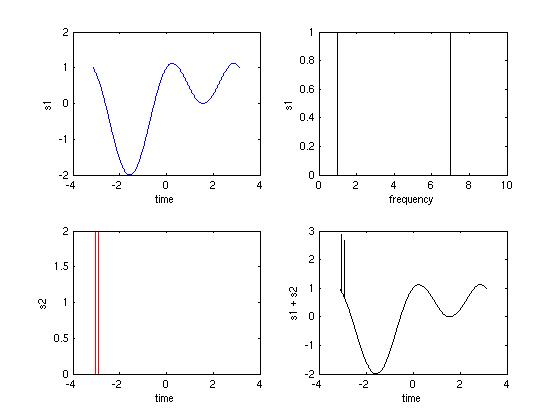
\includegraphics[scale = 0.75]{signalExampleMatlab.jpg}
\caption{The signal s1 has a sparse representation in the frequency domain. s2 has a sparse representation in the time domain. But, the signal (s1 + s2) has a sparse repersentation in an overcompelte basis, but not in either the frequency or time domain alone.}
\label{fig:signalExample}
\end{figure}

\subsection{Basic uncertainty principle}
\begin{theorem}
Let $\Phi$ and $\Psi$ be two orthonormal bases for a vector space. For any vector $s \neq 0$, let $s = \Phi a$ and $s = \Psi b$. Let M = $\max_{i,j}|\dprod{\gf_i, \psi_j}|$. Then:
$$\frac{\norm{a}_0 + \norm{b}_0}{2} \geq \sqrt{\norm{a}_0\norm{b}_0} \geq M^{-1}$$.
\end{theorem}
\begin{proof}
The first inequality comes from the well known AM-GM inequality, so we prove $\sqrt{\norm{a}_0\norm{b}_0} \geq M^{-1}$.

Without loss of generality, suppose that $s^{T}s = 1$.

$$1 = a^{T}\Phi^{T}\Psi b \leq \sum_{i,j} |a_i||\dprod{\gf_i, \psi_j}||b_j| \leq M\sum_i |a_i| \sum_j |b_j|$$

Let $A = \norm{a}_0, B = \norm{b}_0$. From $s^{T}s = 1$, we have that $\sum_i |a_i|^{2} = 1 = \sum_i |b_i|^{2}$. Also, $\forall i: |a_i| \leq 1, |b_i| \leq 1$. So:
 
$$\sum_i |a_i| \leq \sqrt{A}, \sum_i |b_i| \leq \sqrt{B}$$

Substituting this into the earlier inequality, we have $\sqrt{\norm{a}_0\norm{b}_0} \geq M^{-1}$.
\end{proof}

From this, we have the following theorem, whose proof is left as a homework exercise.

\begin{theorem}
If $s = [\Phi\ \Psi]g_1, s = [\Phi\ \Psi]g_2$, then $\norm{g_1}_0 + \norm{g_2}_0 \geq \frac{2}{M}$.
\end{theorem}

From this, we have the following corollary:
\begin{corollary}
Suppose that $s = [\Phi\ \Psi]g_1$, and $\norm{g_1}_0 < M^{-1}$. Then, there does not exist a $g_2$ such that $s = [\Phi\ \Psi]g_2$ and $\norm{g_2}_0 < M^{-1}$.
\end{corollary}


Incoherence is the situation where M is small. Thus, incoherence ensures uniqueness for the sparsest representation. In other words, any other representation will have more non-zeros.

This motivates the following question: If s has a unique sparse representation, how do we find it? The answer to this is explored in the next section.


\section{Sparse Representation using $\ell_1$ minimization}
Suppose we want to find the sparsest $\gamma$ such that $\left[ \Phi \Psi \right] \gamma \; = \; s$.
The set of all feasible $\gamma$ is an affine subspace of $\mathbb{R}^n$. We want to know when
$\ell_1$ minimization gives us the sparsest solution.

\begin{theorem}[Donoho and Huo]
\label{DonohoHuo}
 If $\lVert\gamma\rVert_0 \; < \; \frac{1}{2}(1+\frac{1}{M})$ then $\|\widetilde{\gamma}\|_1 > \|\gamma\|_1$ for all
$\widetilde{\gamma}$ such that $\left[ \Phi \Psi \right] \widetilde{\gamma} = \left[ \Phi \Psi \right] \gamma$
\end{theorem}

\begin{proof}
Let $\|\gamma\|_0 \; < \; \frac{1}{2}(1+\frac{1}{M})$. Consider any
$\widetilde{\gamma}$ such that $\left[ \Phi \Psi \right] \widetilde{\gamma} = \left[ \Phi \Psi \right] \gamma$.
Let $x = \widetilde{\gamma} - \gamma$. Then, we have $\left[ \Phi \Psi \right] x = 0$.\\

$\|\widetilde{\gamma}\|_1 > \|\gamma\|_1$ \\ \\
$\Leftrightarrow \; \displaystyle\sum_{k \in \mbox{\begin{small} supp \end{small}}(\gamma)} \left( |\gamma_k + x_k| -|\gamma_k| \right) + \displaystyle\sum_{k \notin \mbox{\begin{small} supp \end{small}}(\gamma)} |x_k| > 0$\\ \\
$\Leftarrow \; \displaystyle\sum_{k \in \mbox{\begin{small} supp \end{small}}(\gamma)} -|x_k| + \displaystyle\sum_{k \notin \mbox{\begin{small} supp \end{small}}(\gamma)} |x_k| > 0$\\ \\
$\Leftrightarrow \; \frac{\displaystyle\sum_{\mbox{\begin{tiny} ON \end{tiny}}}|x_k|}{\displaystyle\sum_{\mbox{\begin{tiny} ALL \end{tiny}}}|x_k|} \; < \; \frac{1}{2}$\\

\noindent where $\displaystyle\sum_{\mbox{\begin{tiny} ON \end{tiny}}}|x_k| = \displaystyle\sum_{k \in \mbox{\begin{small} supp \end{small}}(\gamma)}|x_k|$ and
$\displaystyle\sum_{\mbox{\begin{tiny} ALL \end{tiny}}}|x_k| = \displaystyle\sum_k |x_k|$.\\

\noindent We want this to be true for all supports of size less than $\frac{1}{2}(1+\frac{1}{M})$ and for all $x$
such that $\left[ \Phi \Psi \right] x = 0$. Let $x\neq 0$ be any such vector and let $i$ be such that
$|x_i| \geq |x_j|$ for all $j$. WLOG, by rescaling, we can assume $x_i=v$ where $v$ is a fixed number.
For this, we have $\displaystyle\sum_{\mbox{\begin{tiny} ON \end{tiny}}}|x_k| \leq \|x\|_0 |v|$.

\begin{eqnarray*}
x = \left[ \begin{array}{r}
             x^\Phi \\
	     x^\Psi \\
            \end{array} \right]\\
\|x\|_1 = \|x^\Phi\|_1 + \|x^\Psi\|_1
\end{eqnarray*}

\noindent WLOG, say $i$ is in the $\Phi$ part.
\begin{eqnarray*}
\Phi x^\Phi = -\Psi x^\Psi \\
x^\Phi = -\Phi^T\Psi x^\Psi
\end{eqnarray*}
\noindent since $\Phi$ is an orthonormal matrix. So we have,
\begin{eqnarray*}
\begin{array}{rl}
      |v| = |x_i| &= | \left[ \Phi^T \Psi \right]_i x^\Psi| \\
		  & \leq M \|x^\Psi\|_1
\end{array}\\
\end{eqnarray*}
\begin{equation*}
 \Rightarrow \|x^\Psi\|_1 \; \geq  \; \frac{|v|}{M}
\end{equation*}

\noindent We also have,
\begin{eqnarray*}
\begin{array}{rl}
  \|x^\Phi\|_1 \; &\geq \; |v| \\ \\
  \Rightarrow \displaystyle\sum_{\mbox{\begin{tiny} ALL \end{tiny}}} |x_k| &= \; \|x\|_1 \; \geq \; |v|\left( 1 + \frac{1}{M}\right)
\end{array}
\end{eqnarray*}

\noindent So for any $x$ such that $\left[ \Phi \Psi \right] x = 0$,
\begin{equation*}
  \frac{\displaystyle\sum_{\mbox{\begin{tiny} ON \end{tiny}}}|x_k|}{\displaystyle\sum_{\mbox{\begin{tiny} ALL \end{tiny}}}|x_k|} \; \leq \; \frac{\|\gamma\|_0}{1+\frac{1}{M}}
\end{equation*}

\noindent and since $\|\gamma\|_0 < \frac{1}{2}\left(1+\frac{1}{M}\right)$, we have

\begin{equation*}
 \frac{\displaystyle\sum_{\mbox{\begin{tiny} ON \end{tiny}}}|x_k|}{\displaystyle\sum_{\mbox{\begin{tiny} ALL \end{tiny}}}|x_k|} \; < \; \frac{1}{2}
\end{equation*}

\noindent proving the result.

\end{proof}

Elad and Bruckstein further refine the sufficient condition to $\|\gamma\|_0 < \frac{\sqrt{2}-\frac{1}{2}}{M}$.
So under these conditions, if we solve $\operatorname{argmin}\; \|\gamma\|_1 \mbox{ s.t. } \left[ \Phi \Psi \right] \gamma=s$,
we are guaranteed to find the unique sparsest solution.

\end{document}

